\documentclass[border=4pt]{standalone}
\usepackage{tikz}
\usepackage{pgfplots}
\pgfplotsset{compat=1.18}
\usetikzlibrary{shapes.geometric,arrows.meta,positioning,calc,fit,decorations.pathreplacing,backgrounds}
\definecolor{boxblue}{RGB}{225,238,252}
\definecolor{boxgreen}{RGB}{225,247,231}
\definecolor{boxorange}{RGB}{253,236,216}
\definecolor{boxgray}{RGB}{237,237,237}
\definecolor{boxred}{RGB}{253,226,226}
\begin{document}
\begin{tikzpicture}[
  box/.style={draw, rectangle, rounded corners, minimum height=0.9cm, minimum width=3.0cm, align=center, font=\footnotesize},
  arr/.style={-{Latex[length=2.5mm]}, thick}
]
\node[box, fill=boxblue] (gasconv) at (0,1.4) {Convezione gas\\ (Cap.\,2)};
\node[box, fill=boxblue] (gasrad) at (0,0.1) {Irraggiamento\\ (Cap.\,3)};
\node[box, fill=boxgray, minimum width=3.4cm] (he) at (4.4,0.75) {$h_e$ (o $h_i$ se gas dentro tubo)};

\node[box, fill=boxgreen] (waterboil) at (8.8,1.4) {Ebollizione/convezione\\ acqua-vapore (Cap.\,4)};
\node[box, fill=boxgray, minimum width=3.4cm] (hi) at (8.8,0.1) {$h_i$ (o $h_e$ se acqua sul mantello)};

\node[box, fill=boxorange, minimum width=7.6cm] (U) at (4.4,-1.6) {$\dfrac{1}{U_k} = \dfrac{1}{h_e}+\dfrac{d_o \ln(d_o/d_i)}{2k_m}+\dfrac{d_o}{d_i}\dfrac{1}{h_i}+R_f$};

\node[box, fill=boxgray, minimum width=6.0cm] (props) at (4.4,-3.0) {Proprietà gas (Cap.\,7) / acqua-vapore (Cap.\,8) alla $T$ locale};

\draw[arr] (gasconv) -- (he);
\draw[arr] (gasrad) -- (he);
\draw[arr] (waterboil) -- (hi);
\draw[arr] (he) -- (U.north -| he);
\draw[arr] (hi) -- (U.north -| hi);
\draw[arr] (props) -- (U);
\end{tikzpicture}
\end{document}
